\documentclass[12pt,a4j]{jreport}
\setcounter{secnumdepth}{5}
\usepackage[dvipdfmx]{graphicx}
\usepackage{amsmath,amssymb}
\usepackage{comment}
\usepackage{graphicx}
\usepackage{here}
\usepackage{bm}
\usepackage{url}
\newcommand{\todo}[1]{{\{\bf todo: #1\}}}

\renewcommand{\baselinestretch}{1.5}

\renewcommand{\bibname}{参考文献}





\begin{document}


%%%%%%%%%%%%%%%%%%%%%%%%%%%%%%%%%%%%%
% 表紙
%%%%%%%%%%%%%%%%%%%%%%%%%%%%%%%%%%%%%
\begin{titlepage}

\begin{center}

    \vspace*{2cm}
    \Large 2023 年度 芝浦工業大学 工学部 情報工学科\\

    \vspace*{1.0cm}
    \Huge 卒 \qquad 業 \qquad 論 \qquad 文\\
    \vspace*{2.5cm}

    %TODO 編集 : 題目
    \Large Standard MLを対象とした不完全な組パターンに対する補完手法の提案および実装
    
    \vspace{4cm}
    \begin{tabular}{ll}
        %TODO 編集 : 題目
        \vspace*{2mm}
        学籍番号 & \qquad $\mathbf{AL20047}$ \\
        \vspace*{2mm}
        氏\phantom{  }名 & \qquad 庄司 \quad 歩夢   \\
        \vspace*{2mm}
        指導教員           & \qquad 篠埜 \quad 功 \\
        \vspace*{2mm}
        提出日 & \qquad 2024年2月
    \end{tabular}
\end{center}
\end{titlepage}




{\makeatletter
\let\ps@jpl@in\ps@empty
\makeatother
\pagestyle{empty}
\tableofcontents
\clearpage}

\setcounter{page}{1} 
\pagestyle{plain}

%%%%%%%%%%%%%%%%%%%%%%%%%%%%%%%%%%%%%%%%%%%%%%%%%%%%%%%%%%%%%
% 序論 
%%%%%%%%%%%%%%%%%%%%%%%%%%%%%%%%%%%%%%%%%%%%%%%%%%%%%%%%%%%%%
\chapter{はじめに}
コード補完機能を利用することで,プログラム開発を効率的に行うことができる.コード補完とは,統合開発環境(IDE)などのコードエディタから利用可能な支援機能で,入力途中のコードに対してその続きを入力する候補を自動表示する機能である.この機能を利用することによって開発者はコードをすべて直接記述する必要がなくなるため,開発の効率を向上させることができる.コード補完機能はEclipse,IntelliJ IDEA,Visual Studio Code等の統合開発環境では標準的に搭載されており,多くの開発者がコード補完を利用しているしているとの調査結果がある\cite{useIDE}.また,補完機能と関連して二つの関連研究を挙げる.三浦\cite{eff}はProcessing言語において初学者がどのようにコード補完を利用するのか調査した結果,補完機能を利用することで括弧の入力数が有意に下がり,補完機能の有用性を示した.石原らは,既存の手法では書きかけのコード中に書き忘れがあった場合にそれらを補完することができないため,書き忘れたコードも補完対象とすることでコード補完の機会がどの程度向上するかについての調査を行った.その結果書き忘れが起こっていた場合でも適切な補完が行われると示した.したがってコード補完はコード開発をするうえで必要である.

しかし,すべてのプログラミング言語に対して補完機能が十分に整っていないのが現状である.実際に,関数型言語のStandard ML\cite{StandardML}はパターンマッチングによって複雑な条件分岐の記述を簡潔に書くことができたり,コンパイル時に型が検査され安全性が高いなどの特徴がありながらも,補完機能が充実していない.それに対して佐藤は\cite{sato},統合開発環境であるVisual Studio Code\cite{vscode}上でStandard MLのサブセット言語を対象にして関数宣言における括弧の記述忘れと引数の記述忘れに対して変数名の補完が行われた.しかし,この研究は括弧の記述忘れと引数の記述忘れという書き間違えが発生していた場合に対して変数名を補完するものであり,括弧を補完したり引数を補完するものではない.したがって本研究では統合開発環境であるVisual Studio CodeでStandard MLを対象とした不完全な組パターンに対する補完手法を提案する.

本論文の構成は次の通りである.まず2章において関連研究について述べる.3章において補完機能の実装概要についてのべる.4章においてに字句解析手法ついて述べる.5章において構文解析手法について述べる.6章において補完候補の取得について述べる.7章において実装方法について述べる.8章において考察を述べる.9章においてまとめと今後の課題を述べる.

%%%%%%%%%%%%%%%%%%%%%%%%%%%%%%%%%%%%%%%%%%%%%%%%%%%%%%%%%%%%%
%%%%%%%%%%%%%%%%%%%%%%%%%%%%%%%%%%%%%%%%%%%%%%%%%%%%%%%%%%%%%
\chapter{関連研究}

関連研究として,コード補完の有用性,書き忘れたコードに対するコード補完,構文誤りを含むソースコードに対するコード補完について本研究との関連性について調査する.

\section{コード補完の有用性}
三浦\cite{eff}は,効率的なプログラミングのために一般的に導入されている補完機能に着目し,初学者がどのように補完機能を利用するかProcessing言語を対象に調査した.その結果,自動補完を活用する学習者とそうでない学習者に二分された.利用頻度の高い補完候補には,for文やif文,画面描画関連の関数呼び出し,およびvoidであった.for文やif文のスニペットには、括弧やカーリーブラケットを含んでいたため,補完機能を利用した編集行為の前後の文と,補完機能を利用しなかった編集行為の前ぼの文と比較すると,括弧やカーリーブラケットの入力数が下がった.そのため,無限ループを生じる記述ミスの回数を有意に減少させることが確認された.しかし,この研究では,補完候補を表示するためにTabを入力しなければならないため,自動補完を活用する学習者が二分化されてしまった.したがって,本研究では補完候補が表示されるべきところで常に表示させるようにすることで,補完が使われないことを防ぐ.


\section{書き忘れたコードに対するコード補完}
石原らは,既存の手法では書きかけのコードの途中に書き忘れがあった場合にそれらを補完することができないため,書き忘れたコードも補完対象とすることでコード補完の機会がどの程度向上するかについて調査した\cite{hos}.この調査実験はJavaで実施され,被検体がタスクを実行していく中で書き忘れがどの程度発生していて,書き忘れに対する補完がどの程度行われたかを調査するものであった.その結果,書き忘れは全タスクのうち約80%で発生しており,その中で最も多い書き忘れはメソッドの引数に関するものであった.また,それらの書き忘れが起こっていたタスクうち24%のタスクにおいて書き忘れたコードに対する適切な補完候補が存在していることを示した.よって本研究で実装しようとしている不完全な組パターンに対する補完も有益であると期待される.

\section{構文誤りを含むソースコードに対するコード補完}
先行研究\cite{sato}では,Standard MLのサブセット言語においてerrorトークンを挿入することで構文誤りが存在しても補完が行われる実装が行われた.実装は統合開発環境であるVScodeでStandard MLのサブセットを対象に,関数宣言による括弧の記述忘れと引数の記述忘れに対して変数名の補完が行われた.本研究では,このサブセット言語を変更して不完全な組パターンに対して補完を行う.




%%%%%%%%%%%%%%%%%%%%%%%%%%%%%%%%%%%%%%%%%%%%%%%%%%%%%%%%%%%%%
%%%%%%%%%%%%%%%%%%%%%%%%%%%%%%%%%%%%%%%%%%%%%%%%%%%%%%%%%%%%%
\chapter{提案手法}

不完全な組パラメータを補完する方法を提案する.
Standard MLのサブセット言語に対して補完を行う.補完は,字句解析,構文解析,補完候補の取得,補完候補の表示の順に行っていく.以下に実際に関数の引数が複数ある際に,括弧の記述を忘れたの補完の例を示す\ref{CodeCompletionDemo}.

\begin{figure}[H]
    \centering
    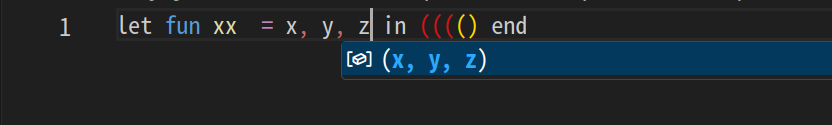
\includegraphics[width=15cm]{img/SampleComplete.png}
    \caption{括弧の補完例}
    \label{CodeCompletionDemo}
\end{figure}

\todo{
    \\
    今回の研究で使うサブセット言語をここに記述\\
    括弧の補完候補のスクリーンショット\\ 
}




\chapter{実装}

\section{VSCode上での補完候補表示}
\todo{
    括弧の補完候補のスクリーンショット
}



%%%%%%%%%%%%%%%%%%%%%%%%%%%%%%%%%%%%%%%%%%%%%%%%%%%%%%%%%%%%%
%%%%%%%%%%%%%%%%%%%%%%%%%%%%%%%%%%%%%%%%%%%%%%%%%%%%%%%%%%%%%
\chapter{字句解析}
字句解析器を生成するプログラムであるFlex\cite{flex}というツールを用いて字句解析を行う.





%%%%%%%%%%%%%%%%%%%%%%%%%%%%%%%%%%%%%%%%%%%%%%%%%%%%%%%%%%%%%
%%%%%%%%%%%%%%%%%%%%%%%%%%%%%%%%%%%%%%%%%%%%%%%%%%%%%%%%%%%%%
\chapter{構文解析}
構文解析器を生成するパーサージェネレーターの1つであるBison\cite{bison}を用いて実装を行う.





%%%%%%%%%%%%%%%%%%%%%%%%%%%%%%%%%%%%%%%%%%%%%%%%%%%%%%%%%%%%%
%%%%%%%%%%%%%%%%%%%%%%%%%%%%%%%%%%%%%%%%%%%%%%%%%%%%%%%%%%%%%
\chapter{補完候補の取得}
Language Serverで補完候補の計算を行う\cite{lsp}.






\chapter{考察}




\chapter{まとめと今後の課題}










\chapter*{謝辞}
\addcontentsline{toc}{chapter}{謝辞}


\newpage
\bibliographystyle{junsrt}
\addcontentsline{toc}{chapter}{参考文献}
\bibliography{ref.bib}


\end{document}
